% Template for ICIP-2018 paper; to be used with:
%          spconf.sty  - ICASSP/ICIP LaTeX style file, and
%          IEEEbib.bst - IEEE bibliography style file.
% --------------------------------------------------------------------------
\documentclass{article}
\usepackage{spconf,amsmath,graphicx, float, hyperref}
\usepackage{amssymb}
\usepackage{pdfpages}

% Example definitions.
% --------------------
\def\x{{\mathbf x}}
\def\L{{\cal L}}

% Title.
% ------
\title{Treinamento e avaliação de generalização do vocoder MelGan \\ \normalsize{Processamento de Linguagem Natural - Prof. Adriano Veloso}}
%
% Single address.
% ---------------
\name{Thiago Malta Coutinho\thanks{Processamento de Linguagem Natural - Prof. Adriano Veloso}}
\address{thiagomaltac@gmail.com}
%
% For example:
% ------------
%\address{School\\
%	Department\\
%	Address}
%
% Two addresses (uncomment and modify for two-address case).
% ----------------------------------------------------------
%\twoauthors
%  {A. Author-one, B. Author-two\sthanks{Thanks to XYZ agency for funding.}}
%	{School A-B\\
%	Department A-B\\
%	Address A-B}
%  {C. Author-three, D. Author-four\sthanks{The fourth author performed the work
%	while at ...}}
%	{School C-D\\
%	Department C-D\\
%	Address C-D}
%
\begin{document}
%\ninept
%
\maketitle
%
\begin{abstract}
Esse trabalho avalia o treinamento da rede Adversarial Generativa MelGan\cite{melgan} em um Corpus em língua portuguesa e sua capacidade de generalização. A avaliação é feita sobre um conjunto de teste contendo dados do Corpus de treinamento e outros Corpus com dados de outras línguas. Os resultados demonstraram que mesmo com uma quantidade relativamente pequena de iterações de treinamento a rede foi capaz de generalizar para outros Corpus contendo diversos locutores, inclusive locutores de gênero diferente da locutora de treino.
\end{abstract}
%
\begin{keywords}
GAN, Generative Adversarial Network, Vocoder, TTS, Text-to-Speech, Natural Language Processing, MelGan
\end{keywords}
%
\section{Introdução}
\label{sec:intro}

\subsection{Text-to-Speech(TTS)}

\begin{figure}[H]
	\begin{minipage}[b]{1.0\linewidth}
		\centering
		\centerline{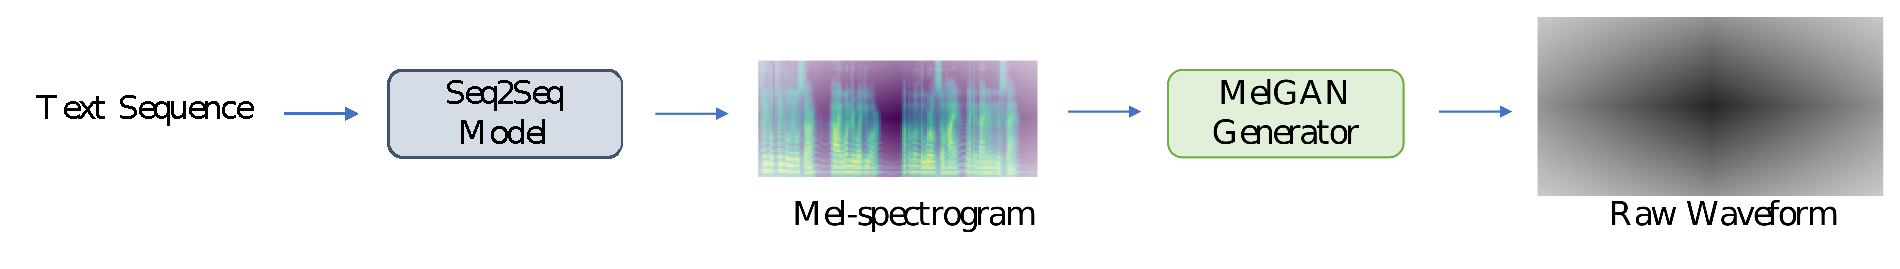
\includegraphics[width=8.5cm]{Figures/tts.eps}}
		%  \vspace{2.0cm}
		\centerline{Result 1}\medskip
	\end{minipage}
	%
	\caption{Problema de geração de áudios a partir de entradas de texto(TTS).}
	\label{fig:res}
	%
\end{figure}

O problema de Text-to-Speech(TTS) consiste em vocalizar áudio a partir de entradas de texto. Até o ano de 2016 as abordagens para o problema eram focadas em modelos concatenativos, que fornecem resultados satisfatórios mas com artefatos de descontinuidade entre fonemas. Em 2016 o modelo WaveNet\cite{wavenet} mostrou que redes neurais são modelos viáveis para o problema de TTS, gerando resultados Estado da Arte(SOTA). 

Os modelos TTS que utilizam redes neurais convergem em uma estrutura em comum contendo duas partes: transformação do texto de entrada para espectrogramas-mel(são gerados a partir de uma transformação baseada no logaritmo, escala que melhor representa a percepção do ouvido humano) e transformação dos espectrogramas para áudios de saída. A primeira etapa é feita por um modelo do tipo \textit{Seq2Seq}, predominantemente o Tacotron-2\cite{tacotron2}. A segunda fase do problema é abordada por outro tipo de modelo, os \textit{Vocoders}. Os \textit{Vocoders} são redes neurais capazes de transformar espectrogramas-mel em áudios, entre as redes presentes na literatura existem redes auto-regressivas\cite{wavenet}\cite{wavernn} e redes não-auto-regressivas\cite{clarinet}\cite{parallelwavenet}\cite{WaveGLOW}.

Em modelos auto-regressivos a inferência da rede possui dependência sequencial e, portanto, produzem áudios com velocidades menores que redes não-auto-regressivas. No entanto inferência em velocidades maiores que tempo real podem ser atingidas. Devido à inferência mais lenta, impossibilitando aplicações de grande porte, modelos não-auto-regressivos tem sido o alvo de novos estudos. 

\section{Metodologia}
\label{sec:format}


\subsection{MelGan}

MelGan\cite{melgan} é uma rede Generativa Adversarial, a ideia é treinar duas redes, uma discriminadora e outra generativa. As duas redes são treinadas em conjunto, uma tentando exercer seu papel melhor que a outra. O objetivo da rede generativa é receber espectrogramas-mel e gerar áudios nos quais a rede discriminativa não consiga distinguir se são reais ou gerados pela rede generativa. O objetivo da rede discriminadora é distinguir entre áudios reais e áudios gerados pela rede adversária, com o menor erro possível. O fim do treinamento acontece quando as duas redes entram em equilíbrio, ou seja, nenhuma das duas consegue melhorar mais. Ao atingir o equilíbrio espera-se que a rede generativa tenha aprendido a gerar saída indistinguíveis das reais, caso a complexidade da rede geradora e discriminadora seja suficiente.

\subsubsection{Rede Geradora}

A rede geradora é totalmente convolucional. Como os espectrogramas-mel possuem dimensão temporal 256x menor que o áudio de saída, camadas de convolução transposta são utilizadas para fazer \textit{upsampling} das amostras de entrada. Cada camada de convolução transposta é seguida por empilhamentos de blocos residuais\cite{wavenet} com convoluções dilatadas. Camadas compostas por \textit{upsampling} e empilhamentos residuais são empilhadas umas sobre as outras para induzir um viés que relaciona amostras temporalmente afastadas. 

\begin{figure}[H]
	\begin{minipage}[b]{0.48\linewidth}
		
		{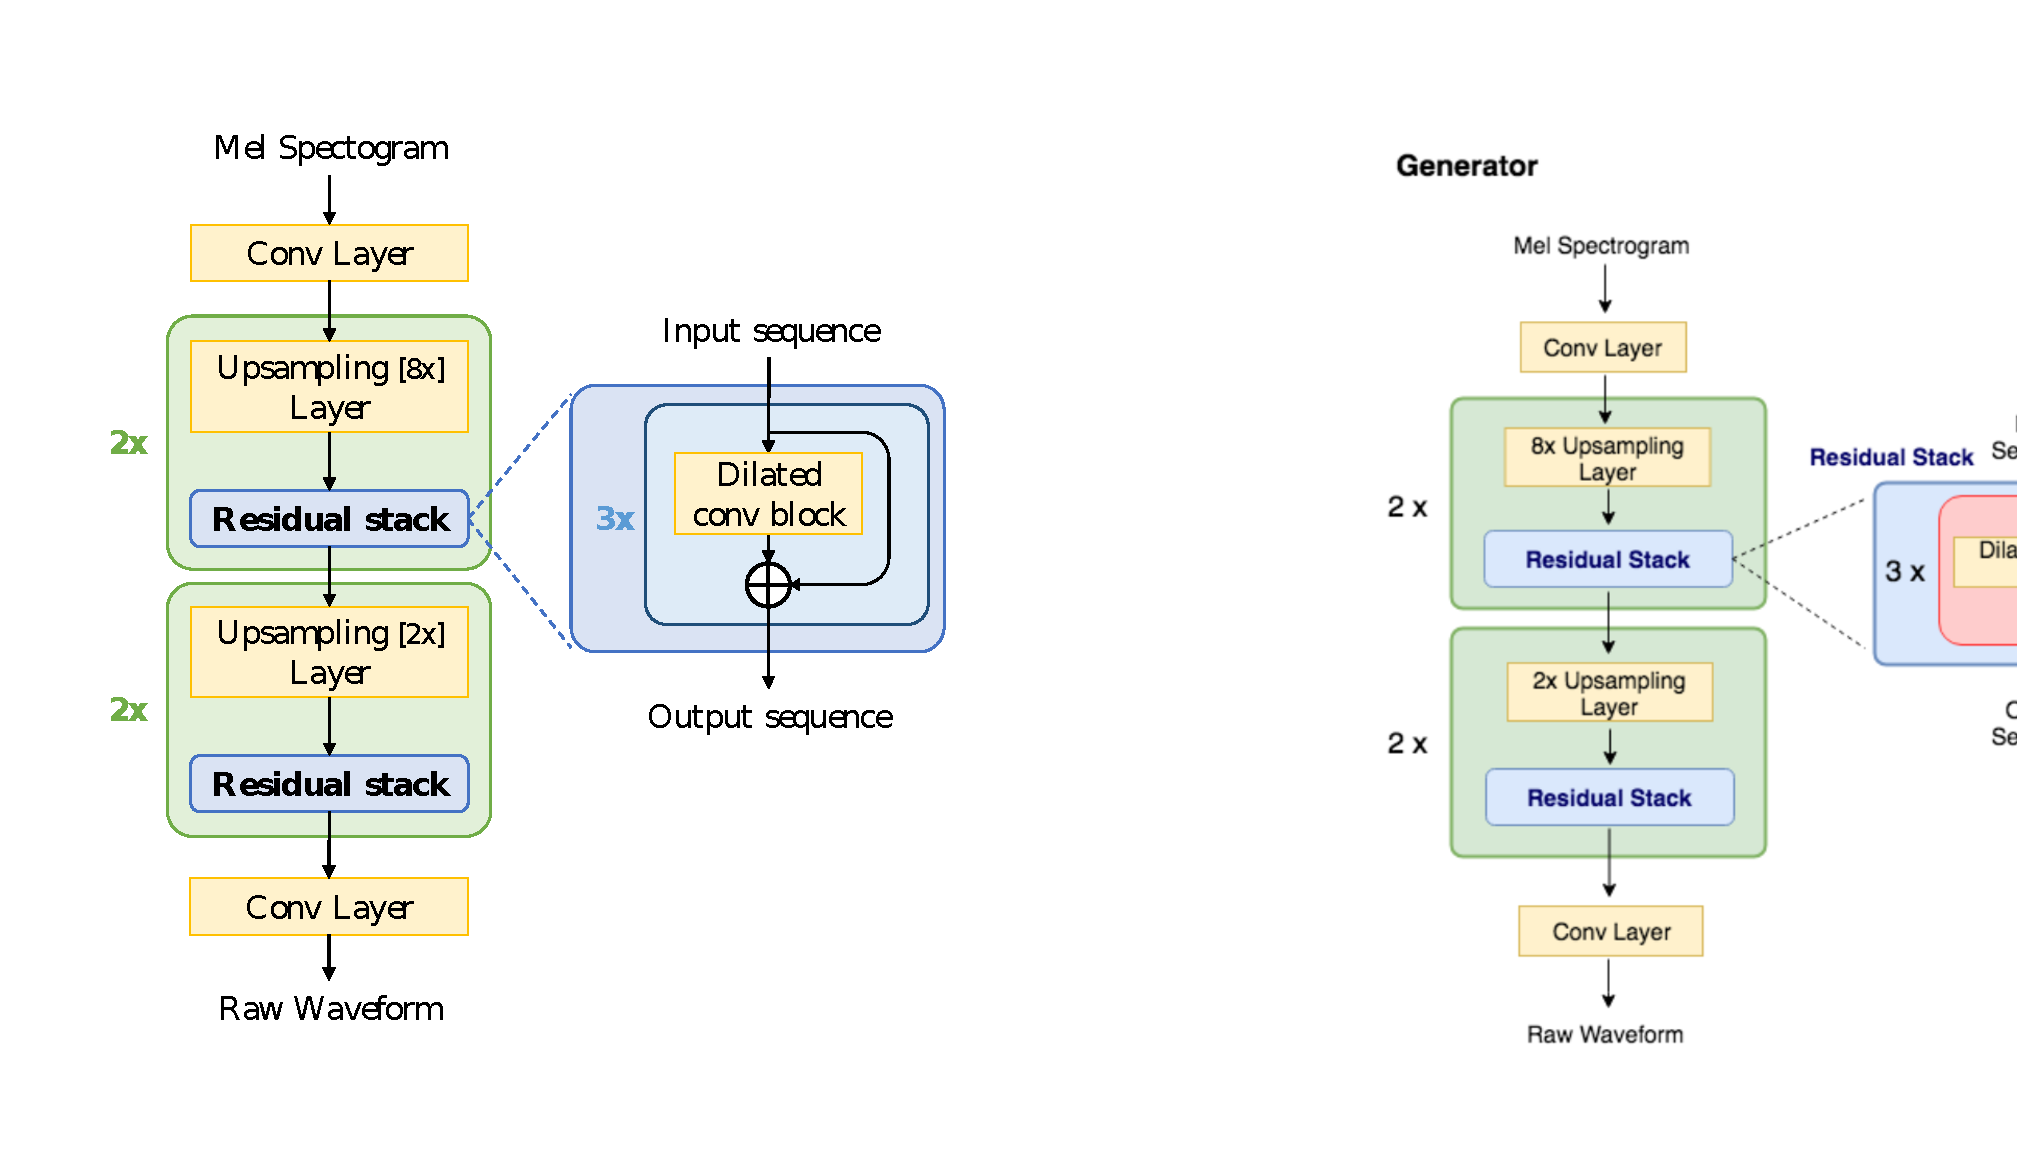
\includegraphics[width=9.5cm]{Figures/gen.eps}}
		%  \vspace{1.5cm}
		\centerline{(a) Camadas do gerador.}\medskip
	\end{minipage}
	\begin{minipage}[b]{.48\linewidth}
		\centering
		\centerline{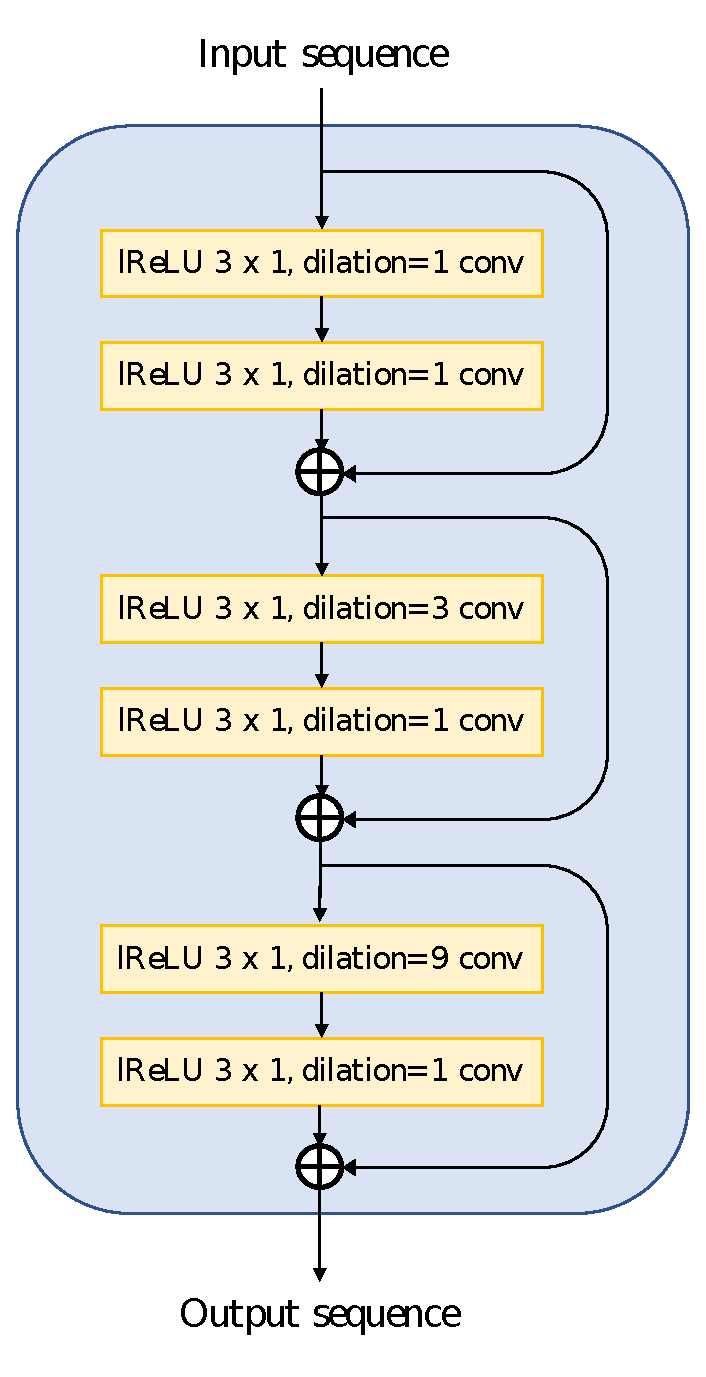
\includegraphics[width=2.5cm]{Figures/res_stack.eps}}
		%  \vspace{1.5cm}
		\centerline{(b) Empilhamentos Residuais.}\medskip
	\end{minipage}
	%
	\caption{Estrutura generativa da rede.}
	\label{fig:res}
	%
\end{figure}

Para as camadas de convolução transpostas os autores utilizaram tamanho de kernel divisível pelo stride, para evitar os \textit{Checkerboard Artifacts}\cite{checkerboard-artifacts}. Para cada camada da rede geradora, os autores utilizam \textit{Weight Normalization}\cite{weightnorm}, uma reparametrização dos pesos da rede:

\begin{equation}
\textbf{W} = \frac{g}{||\textbf{v}||}\textbf{v} \implies ||\textbf{W}|| = g
\end{equation}

\subsubsection{Rede Discriminadora}

\begin{figure}[H]
	\begin{minipage}[b]{1.0\linewidth}
		\centering
		\hspace*{-4.3cm}
		{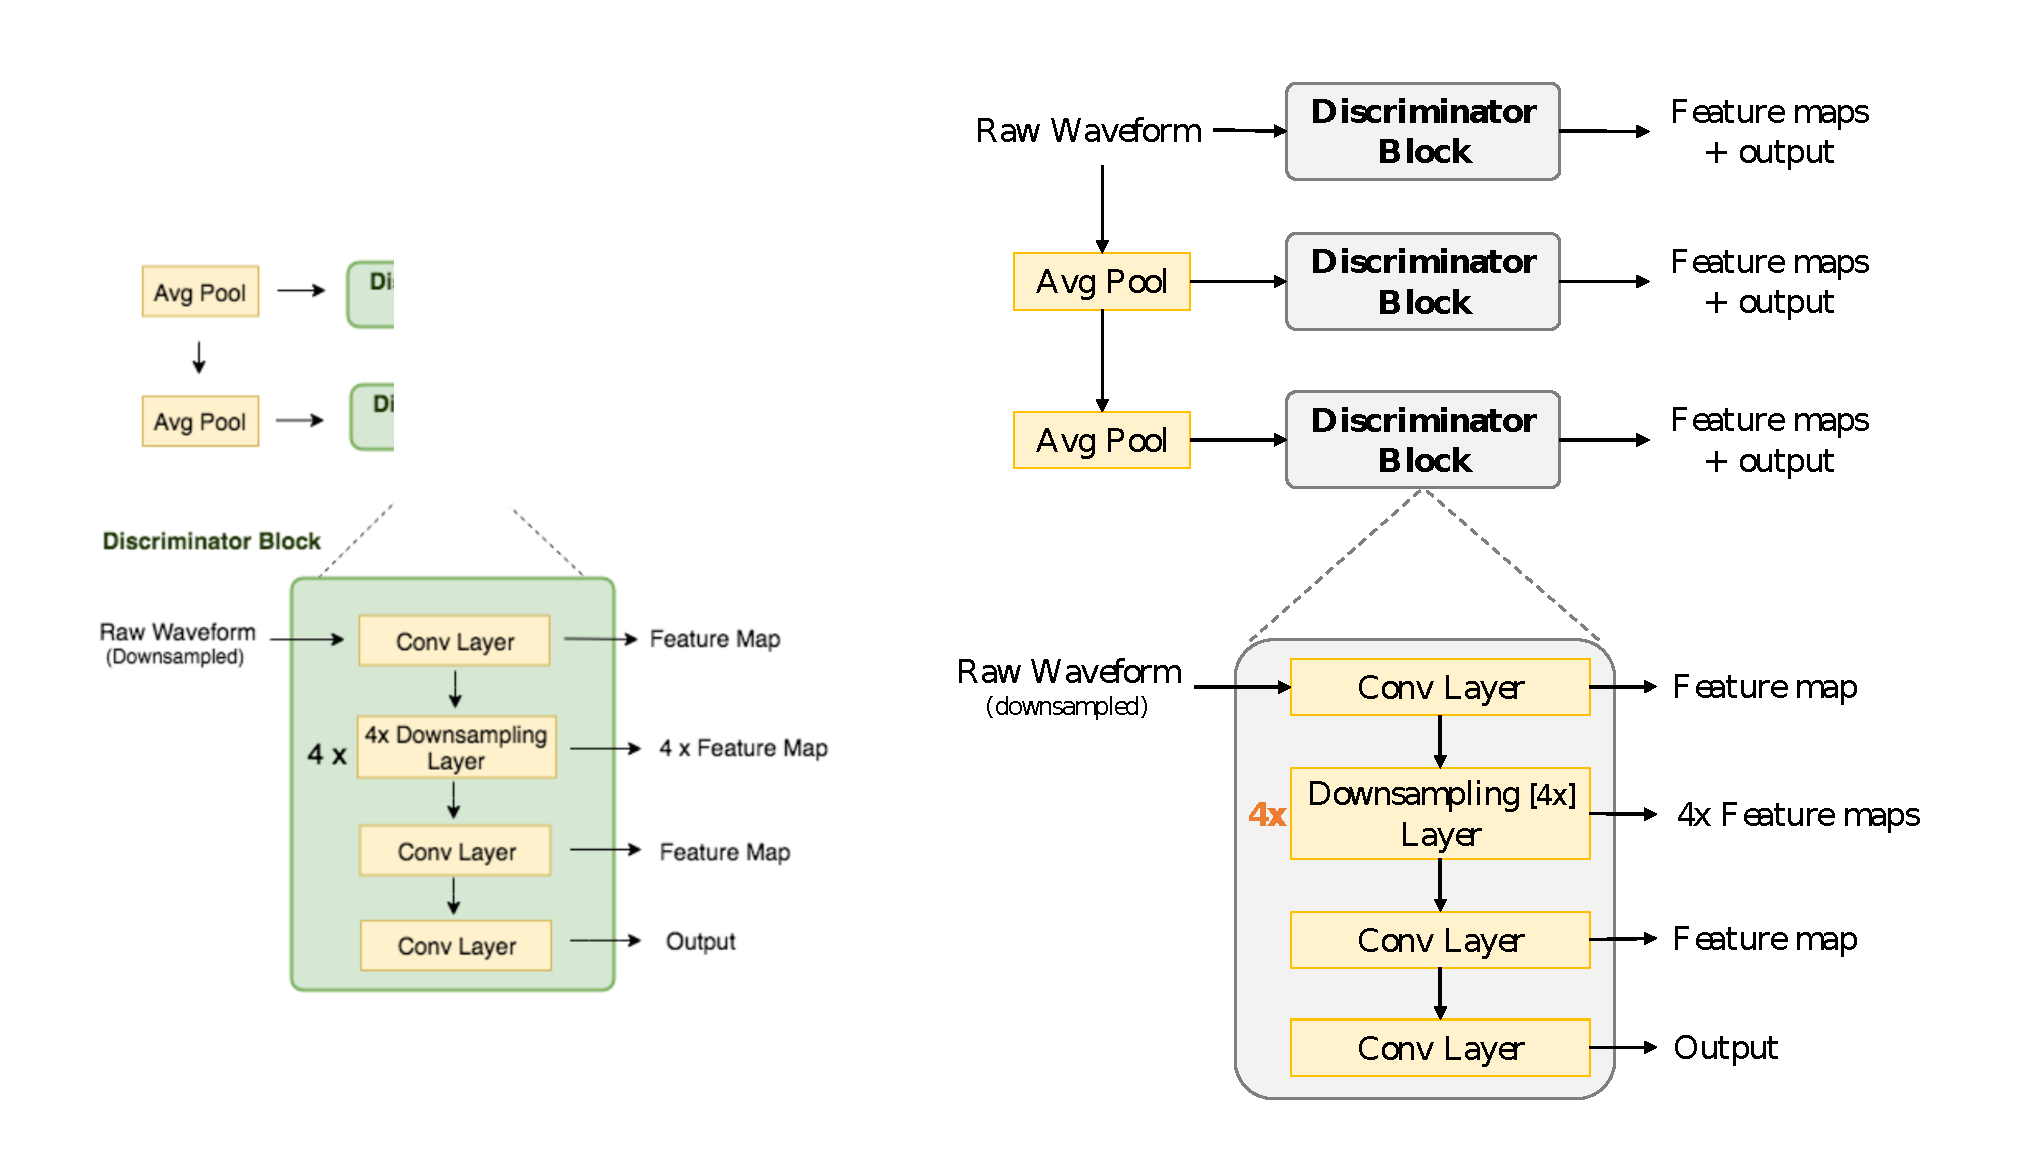
\includegraphics[width=8.5cm]{Figures/dis.eps}}
		%  \vspace{2.0cm}
	\end{minipage}
	%\hspace{\fill}
	%
	\caption{Estrutura do discriminador com o detalhamento do bloco discriminador.}
	\label{fig:res}
	%
\end{figure}

A rede discriminadora possui três discriminadores com estrutura idêntica mas operando em diferentes frequências temporais. O primeiro discriminador opera sobre o sinal de áudio puro, o segundo sobre o sinal amostrado por um fator de 2 e o terceiro por um fator de 4. Os autores justificam a abordagem dizendo que os áudios possui informação em diferentes níveis. Portanto cada discriminador aprende características para diferentes faixas de frequência do áudio. Operar apenas com um discriminador no áudio puro iria introduzir um viés resultando no aprendizado apenas de \textit{features} baseadas em componentes de baixa frequência.

\subsubsection{Funções objetivo}

Os autores usaram como função objetivo a versão da \textit{Hinge Loss}\cite{} para GAN's: 

\begin{equation}
\min_{D_k} \mathbb{E}_x \Big[\min(0, 1 - D_k(x))\Big] + \mathbb{E}_{s,z} \Big[\min(0, 1 + D_k(G(s, z)))\Big],\  \forall k\\
\end{equation}

\begin{equation}
\min_G \mathbb{E}_{s,z} \Bigg[\sum_{k=1,2,3}-D_k(G(s, z)) \Bigg]
\end{equation}

Além do sinal do discriminador, os autores utilizam uma função de perda com \textit{Feature Matching}\cite{} para a função objetivo do gerador. O objetivo é minimizar a distância L1 entre o \textit{feature map} do discriminador para áudios reais e sintéticos.

\begin{equation}
\mathcal{L}_{\text{FM}}(G, D_k) = \mathbb{E}_{x, s \sim p_\text{data}} \Bigg[\sum_{i=1}^T \frac{1}{N_i} ||D_k^{(i)}(x) - D_k^{(i)}(G(s))||_1\Bigg]
\end{equation}

Assim, função de perda do gerador é dada por:

\begin{align}
\min_G \Bigg(\mathbb{E}_{s,z} \bigg[\sum_{k=1,2,3} -D_k(G(s, z)) \bigg] + \lambda \sum_{k=1}^3 \mathcal{L}_{\text{FM}}(G, D_k) \Bigg)
\end{align}

\subsection{Corpus}

O Corpus utilizado foi obtido nas bibliotecas abertas LibriVox\cite{librivox} e Projeto Gutenberg\cite{gutenberg}. Os áudios e texto foram são do livro A Relíquia, de Eça de Queirós, o áudio está disponível em \cite{reliquia} e o texto em \cite{reliquia-text}. O Corpus contém 10 horas e 31 minutos de áudio, com locutora feminina falando em língua portuguesa do Brasil. Os arquivos de áudio vem particionados em pedaços que variam entre oito minutos e uma hora.

\subsection{Pré-processamento dos dados}

Para a rede aprender com mais eficácia, os áudios a serem aprendidos devem ter duração máxima até 30 segundos, áudios maiores são mais difíceis de modelar devido à duração. A partir dessa premissa, os arquivos de áudio do Corpus foram particionados para tamanhos menores. 

Para realizar a tarefa de maneira automatizada o alinhamento do texto com o áudio foi feito a partir de uma rotina baseada no algoritmo Virtebi. Os caracteres especiais do tipo UTF-8 foram removidos do texto, junto com parêntesis e traços, os acentos foram substituídos por texto comum para facilitar o alinhamento. Como o texto vem separado com quebra de linhas em frases e parágrafos, os áudios cortados teriam tamanho próximo ao desejado.

\begin{figure}[H]
	\begin{minipage}[b]{1.0\linewidth}
		\centering
		\centerline{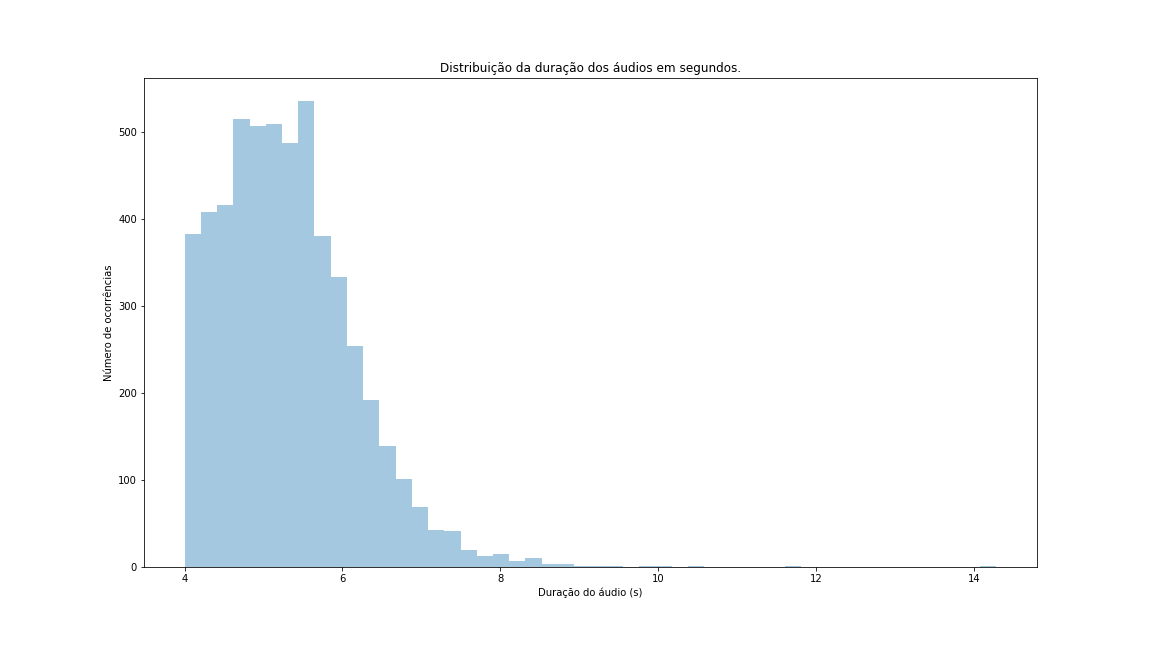
\includegraphics[width=8.5cm]{Figures/dist_duracao.png}}
		%  \vspace{2.0cm}
	\end{minipage}
	\caption{Distribuição da duração dos áudios do Corpus.}
	\label{fig:DistAudios}
\end{figure}

Após o particionamento dos áudios, os arquivos com duração menor que quatro segundos foram filtrados para garantir um tamanho mínimo. A Figura \ref{fig:DistAudios} mostra a distribuição final da duração dos áudios do Corpus. O arquivo com maior duração tem 14 segundos, o menor tem 4 segundos e a média está em 5,3 segundos. A duração total do Corpus foi reduzida para 7 horas e 57 minutos, com 5.397 arquivos de entrada.

\subsection{Treinamento}


A rede foi treinada por 957 mil iterações com os hiper parâmetros especificados na Tabela \ref{tab:hiperparams}.

\begin{table}[H]
	\centering
	\begin{tabular}{|l|l|}
		\hline
		Parâmetro & Valor \\ \hline
		Número de blocos discriminadores & 3 \\ \hline
		Número de camadas residuais & 3 \\ \hline
		Fator de Downsampling & 4 \\ \hline
		Número de canais mel & 80 \\ \hline
		$\lambda$ & 10 \\ \hline
		Tamanho do Batch & 16 \\ \hline
	\end{tabular}
	\caption{Hiper parâmetros utilizados na rotina de treinamento da rede.}
	\label{tab:hiperparams}
\end{table}

Em \cite{melgan} os autores treinam o algoritmo por 2,5M iterações, até a convergência. 

\subsection{Avaliação do desempenho do modelo}

A avaliação do desempenho do modelo é feita qualitativamente nos áudios gerados pela rede, uma métrica de avaliação é o MOS(\textit{Mean Opinion Score}), uma pesquisa de avaliação qualitativa com embasamento estatístico feita com um grande número de ouvintes. 

Para avaliar a generalização do modelo um Corpus de teste foi construído a partir de áudios de diferentes Corpus. A estrutura dos dados está descrita na Tabela\ref{tab:corpus}:

\begin{table}[H]
	\centering
	\begin{tabular}{|l|l|l|l|}
		\hline
		Número de Amostras & Gênero do(a) Locutor(a) & Língua & Ref. \\ \hline
		15 & Feminino & PT-BR & \cite{reliquia} \\ \hline
		8 & Feminino & EN-US & \cite{ljspeech} \\ \hline
		3 & Feminino & PT-BR & \cite{inglaterra} \\ \hline
		8 & Masculino & PT-BR & \cite{inglaterra} \\ \hline
		4 & Feminino & PT-PT & \cite{contos} \\ \hline
		4 & Feminino & PT-BR & \cite{defunto} \\ \hline
	\end{tabular}
	\caption{Composição do Corpus de teste.}
	\label{tab:corpus}
\end{table}


\section{Resultados}
\label{sec:pagestyle}

\begin{figure}[H]
	
	\begin{minipage}[b]{1.0\linewidth}
		\centering
		\centerline{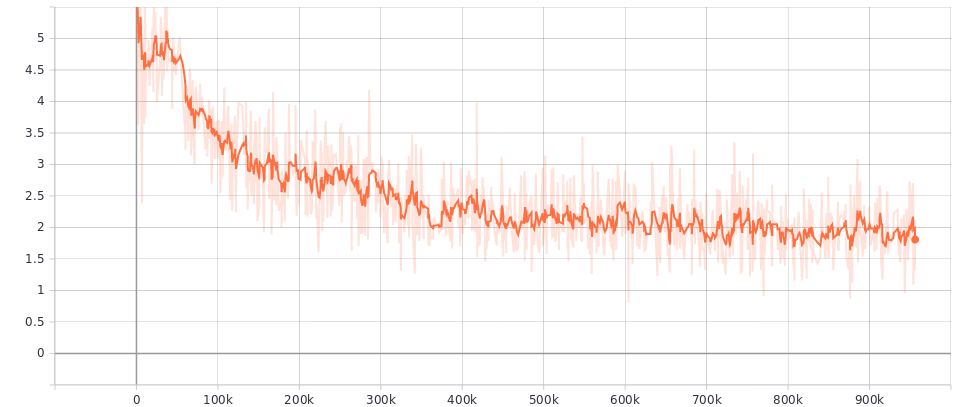
\includegraphics[width=8.5cm]{Figures/discriminator_loss.png}}
		%  \vspace{2.0cm}
		\centerline{(a) Loss do discriminador.}\medskip
	\end{minipage}
	%
	\begin{minipage}[b]{1\linewidth}
		\centering
		\centerline{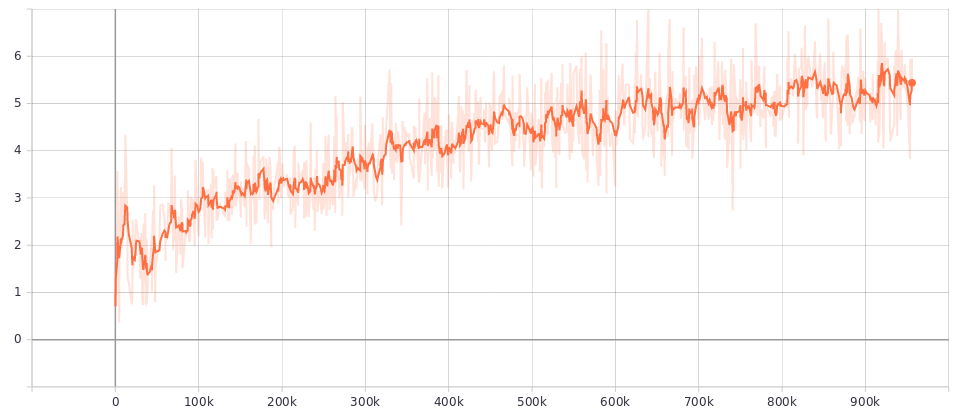
\includegraphics[width=8.5cm]{Figures/generator_loss.png}}
		%  \vspace{1.5cm}
		\centerline{(b) Loss do gerador.}\medskip
	\end{minipage}
	
	\begin{minipage}[b]{.48\linewidth}
		\centering
		\centerline{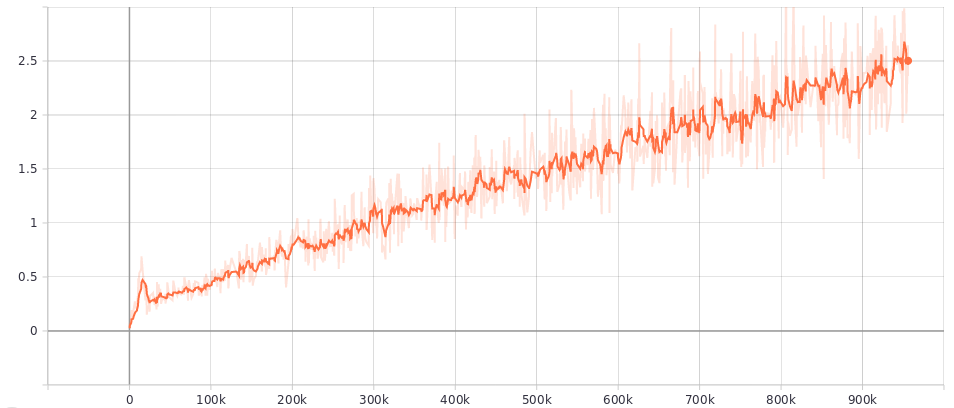
\includegraphics[width=4.0cm]{Figures/feature_matching.png}}
		%  \vspace{1.5cm}
		\centerline{(c) Loss do Feature Matching.}\medskip
	\end{minipage}
	\hfill
	\begin{minipage}[b]{0.48\linewidth}
		\centering
		\centerline{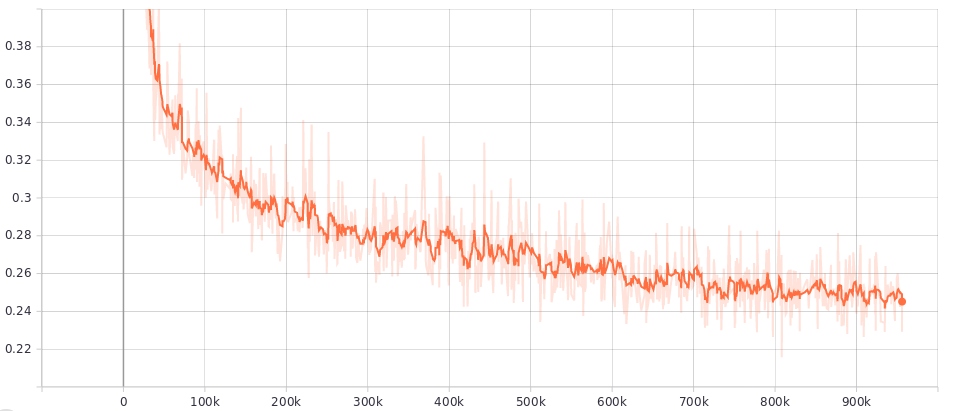
\includegraphics[width=4.0cm]{Figures/mel_reconstruction.png}}
		%  \vspace{1.5cm}
		\centerline{(d) Loss do espectrograma-mel.}\medskip
	\end{minipage}
	%
	\caption{Funções de perda do treinamento da rede MelGan.}
	\label{fig:res}
	%
\end{figure}

As funções de perda do discriminador e gerador apresentaram as características esperadas, uma é similar ao inverso da outra. Além disso, nenhuma rede apresentou crescimento ou decrescimento abrupto na função de perda, podendo gerar \textit{Mode Collapse}. A função de perda da reconstrução do espectrograma-mel(definida pela distância L1 entre a reconstrução do espectrograma e o original), decresceu com o aumento das iterações de treinamento. A loss do \textit{Feature Matching} apresentou característica de crescimento constante.

\section{Conclusões}
\label{sec:typestyle}

Esse trabalhou explorou o treinamento do vocoder MelGan e analisou qualitativamente os resultados obtidos em um Corpus com diferentes locutores em 3 línguas. 

Apesar do número de iterações de treino da rede ser consideravelmente menor que o recomendado pelos autores do modelo\cite{melgan}, a rede apresentou resultados satisfatórios. Os áudios gerados a partir de espectrogramas da mesma locutora do conjunto de treinamento apresentaram poucos artefatos e som limpo. Para outros locutores os áudios apresentaram mais artefatos e qualidade baixa, no entanto os sons são inteligíveis e demonstram a capacidade de generalizar e característica generativa da rede. 


% -------------------------------------------------------------------------


% To start a new column (but not a new page) and help balance the last-page
% column length use \vfill\pagebreak.
% -------------------------------------------------------------------------
%\vfill
%\pagebreak


% References should be produced using the bibtex program from suitable
% BiBTeX files (here: strings, refs, manuals). The IEEEbib.bst bibliography
% style file from IEEE produces unsorted bibliography list.
% -------------------------------------------------------------------------
\bibliographystyle{IEEEbib}
\bibliography{refs}

\end{document}
